\section{Tests of Independence}
\label{sec:independencia}

\subsection{Returning to our example...}
The number of degrees of freedom is the number of categories minus one. In our example $\nu = 2-1 =1.$ Assume a significance level $\beta=0.05.$

\begin{figure}
	\centering
	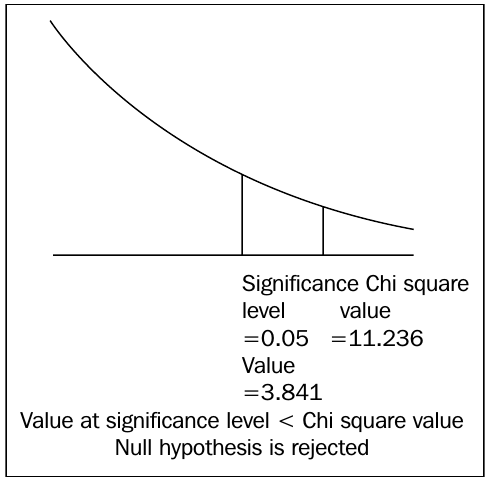
\includegraphics[height=5cm,keepaspectratio=true]{./images/kum0407.png}
	% kum0407.png: 0x0 pixel, 300dpi, 0.00x0.00 cm, bb=
	\caption{The null hypothesis is rejected because the calculated $\chi^2$ statistic exceeds the critical value at the chosen significance level.}
	\label{fig:3.9.2}
\end{figure}

Let us examine another example where we want to demonstrate that a student's gender and the subjects they choose are independent.

Suppose for a group of students, the following table represents the number of men and women taking mathematics, arts, and commerce as their main subjects.

\begin{center}
	\begin{tabular}{|l|l|l|l|l|}\hline
		& Mathematics & Arts & Commerce & Total\\\hline
		Men & 68 & 52 & 90 & 210\\\hline
		Women & 28 & 37 & 35 & 100\\\hline
		Total & 106 & 89 & 125 & 310\\\hline
	\end{tabular}
\end{center}

If gender were not relevant in subject choice, then the expected number of men and women taking the different subjects would be:
\begin{center}
	\begin{tabular}{|l|l|l|l|l|}\hline
		& Mathematics & Arts & Commerce & Total\\\hline
		Men & 71.81 & 60.29 & 84.90 & 210\\\hline
		Women & 34.19 & 28.71 & 40.10 & 100\\\hline
		Total & 106 & 89 & 125 & 310\\\hline
	\end{tabular}
\end{center}

The expected values are calculated as $E_{ij} = \frac{(\text{Row Total}_i)(\text{Column Total}_j)}{\text{Grand Total}}$:
\begin{align}
	E_{11} &= \frac{210 \times 106}{310} = 71.81 \\
	E_{12} &= \frac{210 \times 89}{310} = 60.29 \\
	E_{13} &= \frac{210 \times 125}{310} = 84.90 \\
	E_{21} &= \frac{100 \times 106}{310} = 34.19 \\
	E_{22} &= \frac{100 \times 89}{310} = 28.71 \\
	E_{23} &= \frac{100 \times 125}{310} = 40.10
\end{align}

The deviations are calculated using the formula $(O-E)^2/E$:
\begin{center}
	\begin{tabular}{|l|l|l|l|l|}\hline
		& Mathematics & Arts & Commerce & Total\\\hline
		Men & 0.20 & 1.13 & 0.31 & 1.64\\\hline
		Women & 0.42 & 2.38 & 0.65 & 3.45\\\hline
		Total & 0.62 & 3.51 & 0.96 & 5.09\\\hline
	\end{tabular}
\end{center}

For example, for men in mathematics:
\begin{align}
	\frac{(O-E)^2}{E} = \frac{(68-71.81)^2}{71.81} = \frac{(-3.81)^2}{71.81} = \frac{14.52}{71.81} \approx 0.20
\end{align}

The $\chi^2$ statistic is obtained by summing all these values.

\subsection{Conclusions (from the instructor)}
Since $\chi^2= 4.99$ and the critical value of the $\chi^2$ statistic at the given significance level with $\nu=(2-1)(3-1)=2$ degrees of freedom is $5.991$ (or using $\alpha=0.05$), the null hypothesis is not rejected.

Equivalently,
\begin{align}
	\texttt{p-value}=1- F_{\chi^{2}}(4.99)=0.0825>\beta=0.05,
\end{align}
we arrive at the same conclusion:
\begin{center}
	\emph{Subject choice is independent of gender.}
\end{center}
